\documentclass[main.tex]{subfiles}
\begin{document}
\section{Spherical Pendulum}\label{sec:sphericalpendulum} 
This example was used to motivate the Noether-like theorem in McCarthy's paper. The mechanical system as described in the article is modeled and simulated using the Matlab program.

\textbf{Description} 
A point mass $m_1$ on the $xy$-plane can be actuated in the radial and tangential components $(\rho,\theta)$. Attached to $m_1$ is a rigid massless rod of fixed length $\ell$ with another point mass $m_2$ at the end. The second mass $m_2$ is on or above the $xy$-plane, and is free to move in the azimuthal and tangential components $(\phi,\psi)$.
%Consider a massive body which rotates around a fixed point in space. A leg extends from the body, which can rotate relative to the body and change its length.
\begin{figure}[h]
    \centering
    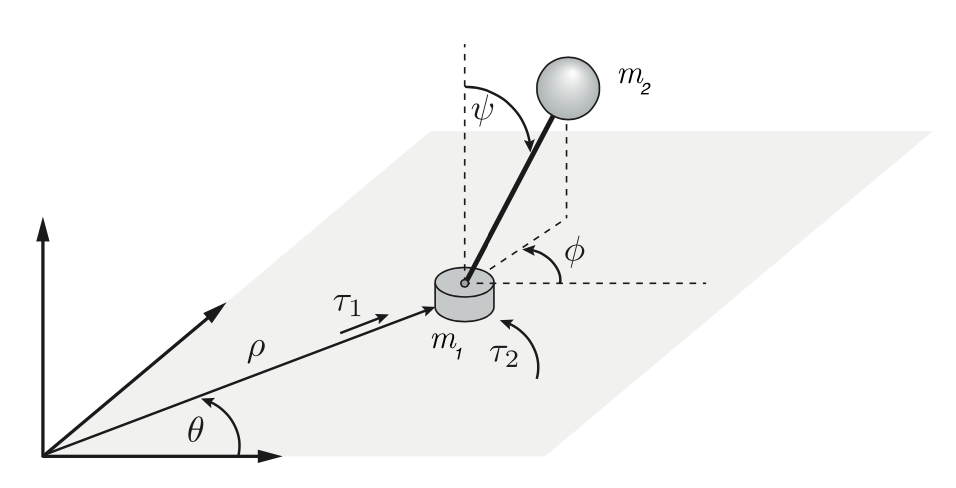
\includegraphics[width=0.8\textwidth]{assets/spherical-pen.png}
    \caption{Schematic diagram of spherical pendulum system \cite[5]{mccarthy}}
    \label{fig:sph-pen}
\end{figure}

\begin{enumerate}[(1)]
\item The smooth simple simple mechanical control system $(Q,\mathbb{G},F,P)$ is defined by:
\begin{itemize}
    \item \textbf{Configuration manifold} $Q=\ree_{>0}\cross\mathbb{S}^1\cross\mathbb{S}^2$, with coordinates $q=(\rho,\theta,\phi,\psi)$.
    \item \textbf{Kinetic metric} $\mathbb{G}=\frac{1}{2}m_1\dot{x}_1^2+\frac{1}{2}m_2\dot{x}_2^2$
    \item \textbf{Actuation} $F=(\dd \rho,\dd \theta)$
    \item \textbf{Potential} $P=-gm_2z=-gm_2(\ell\cos \psi)$
\end{itemize}
From the diagram of the system, it can be shown that the spatial coordinates are
\begin{align}
    \Vec{x}_1&=\pmqty{\rho\sin\theta\\\rho\cos\theta\\0}
    ,\\
    \Vec{x}_2&=\Vec{x}_1+\pmqty{\sin\psi\cos\phi\\\sin\psi\sin\phi\\\cos\psi}
    .
\end{align}
The corresponding velocities are given by,
\begin{align}
    \dot{\Vec{x}}_1&=\pmqty{\rho\dot\theta\cos\theta+\dot\rho\sin\theta\\-\rho\dot{\theta}\sin\theta+\dot\rho\cos\theta\\0}
    ,\\
    \dot{\Vec{x}}_2&=\dot{\Vec{x}}_1+\ell\pmqty{\dot\psi\cos\psi\cos\phi-\dot\phi\sin\psi\sin\phi\\\dot\psi\cos\psi\sin\phi+\dot\phi\sin\psi\cos\phi\\-\dot\psi\sin\psi}. 
\end{align}
\item The system's Lagrangian depends on the kinetic energies and potentials of each point mass. 

The kinetic energy of mass $m_1$ is:
\begin{align}
    G_1(\qd)&=\frac{1}{2}m_1\dot{x}_1^2=\frac{1}{2}m_1
    \del{\rho^2\dot{\theta}^2+\dot{\rho}^2}
    .
\end{align}
The kinetic energy of mass $m_2$ works out to be:
\begin{align}
    G_2(\qd)&=\frac{1}{2}m_2\dot{x}_2^2\\
&\begin{aligned}
{}=\frac{1}{2}m_2&\bigg[
\del{\rho^2\dot{\theta}^2+\dot{\rho}^2}\\
&+\rho\ell\dot{\theta}
\del{
    \dot{\psi}\cos\theta\cos\psi\cos\phi-\dot{\phi}\cos\theta\sin\psi\sin\phi-\dot{\psi}\sin\theta\cos\psi\sin\phi-\dot{\phi}\sin\theta\sin\psi\cos\phi
}\\
&+\ell^2\del{
    \dot{\psi}^2+\sin^2\psi\dot{\phi
}^2
}\bigg]
\end{aligned}
\end{align}
Finally, the potential energy is:
\begin{align}
    P(q) = -gm_2\ell\cos\psi
\end{align}
Finally, we put the pieces together to obtain the Lagrangian of the system. The simplified result is given by,
\begin{align}
    \begin{aligned}
    \Lagr(q,\qd)=
    \frac{1}{2}&\del{m_1+m_2}\del{\rho^2\dot{\theta}^2+\dot{\rho}^2}\\
    & +m_2\rho\ell\dot{\theta}\del{\dot{\psi}\cos\psi\cos(\theta+\phi)-\dot{\phi}\sin\psi\sin(\theta+\phi)}\\
    &+\frac{1}{2}m_2\ell^2\del{\dot{\psi}^2+\sin^2\psi\dot{\phi}^2}\\
    &-gm_2\ell\cos\psi.
    \end{aligned}
    \label{eq:sphericallagr}
\end{align}
\item From Equation \ref{eq:sphericallagr}, the system's symmetry is found to be in the sum $\xi:=\theta+\phi$. 
 % We can therefore equivalently define the Lagrangian using $\xi$ (noting that the velocities $\dot q=(\dot\rho,\dot\theta,\dot\psi)$ are \textit{not} subject to this symmetry):
 % \begin{align}
 %     \Lagr(q,\dot q)&=\Lagr(\rho,\theta,\psi,\dot q)
 %     =\Lagr(\rho,\xi,\dot q).\label{eq:xilagrangian}
 % \end{align}
Define the left action of the Lie group $\mathbb{S}^1$ to be $\Phi:Q\cross \mathbb{S}^1\to Q$ to be the symmetry of the system, where the configuration space is $Q=\ree^+\cross \mathbb{S}^1\cross \mathbb{S}^1$.
%\todoformat[not sure which style to pick]
    \begin{align}
        %\Phi:\del{\pmqty{\rho\\\theta\\\psi},g}\mapsto\pmqty{\rho\\\theta+g\\\psi+g}.\\
        \Phi_\pm:\pmqty{\rho\\\theta\\\phi\\\psi}\in Q,g\in G\mapsto\pmqty{\rho\\\theta\pm g\\\phi\mp g\\\psi}\in Q.
    \end{align}
We can see that for all $g\in G$, this symmetry has no effect on $\xi$:
\begin{align}
    &\xi(q):=\theta+\phi,\\
    &\xi\del{\Phi_\pm(q,g)}=(\theta\pm g)+(\phi\mp g)=\theta+\phi \pm g \mp g=\xi(q).\ \checkmark
\end{align}
Since the Lagrangian's $\theta,\phi$ dependency can be expressed as a function of $\xi$, the Lagrangian is also invariant under the action of $\Phi$.



\item McCarthy chose the following VHCs for this problem,
\begin{align}
    h_1(q)&:=\theta-\psi,\\
    h_2(q)&:=\psi-\frac{\pi}{4}\tanh\rho,
\end{align}
from which we get
\begin{align}
    \dhq&=\pmqty{ 
    0 & 1 & -1 & 0\\
    \frac{\pi}{4}\tanh^2(\rho)-\frac{\pi}{4} & 0 & 0 & 1 },\\
    \Ker{\dhq}&=\cbr{
     \pmqty{ 0\\1\\-1\\0},\pmqty{ 1\\ 0\\ 0\\ -\frac{\pi}{4}\tanh^2(\rho)+\frac{\pi}{4} }}.\label{eq:kerdhqspeherical}
\end{align}

The set of chosen VHCs $h(q)$ (Definition \ref{thm:regularvhc}) constrain the system to a submanifold $\mathcal{C}\subset Q$, with
    \begin{align}
        T_q\mathcal{C}&:=\Ker{\dhq}.\label{eq:tangentspaceqcspherical}
    \end{align}
This tangent space can equivalently be defined using the Ehresmann connection. 
    \begin{align}
        T_q\mathcal{C}=\Span{V(q),H(q)}.
    \end{align}

Take $V(q)$ as the Vertical Vector Field defined by the direction of the symmetry:
    \begin{align}
        V(q):=&\pdv{\Phi_\pm}{g}=\pdv{}{g}\pmqty{\rho\\\theta\pm g\\\phi\mp g\\\psi}=\pmqty{0\\\pm1\\\mp1\\0}\overset{\mathrm{\tiny WLOG}}{=}\pmqty{0\\1\\-1\\0}.\label{eq:dPhidgspherical}
    \end{align}

    The robot arm system has 4 degrees of freedom and 2 actuators, equating to $4-2=2$ degrees of underactuation. Since we plan to use this actuator to enforce the VHC, the constraint manifold should have $\dim\mathcal{C}=2$ remaining degrees of freedom.

    Since $V(q)$ in Equation \ref{eq:dPhidgspherical} also appears in the basis for $T_q\mathcal{C}$ (see Equation \ref{eq:kerdhqspeherical}), it is natural to choose the horizontal component as the second element
    \begin{align}
    H(q)=\pmqty{1\\0\\0\\-\frac{\pi}{4}\tanh^2(\rho)+\frac{\pi}{4}},
    \end{align}
    and their direct sum defines the fiber bundle $T\mathcal{C}=TV\oplus TH$.
    \item 
    The constrained dynamics are computed using the expression with constrained Christoffel Symbols in Equation \ref{eq:constr-dyn-gammac}. 
    
    The Christoffel Symbols (Definition \ref{eq:christoffelconstrained}) of the constraint manifold $\Gammac{k}{ij}$ are computed in Matlab.
    \end{enumerate}
\end{document}